%%==================================================
%% main.tex for BIT Master Thesis
%% version: 0.1
%% last update: Nov 8th, 2017
%%==================================================

% 默认单面打印 oneside 、硕士论文模板 master

\documentclass[oneside, master]{BIT-thesis-grd}

% 打印选项: 双面打印 oneside;单面打印 twoside
% 模板选项: 硕士论文 master; 博士论文 doctor
\graphicspath{{figures/}}

\usepackage{algorithmic}
%\usepackage[ruled]{algorithm2e}
\renewcommand{\algorithmicrequire}{\textbf{输入:}}  
\renewcommand{\algorithmicensure}{\textbf{输出:}}  
\begin{document}

%%%%%%%%%%%%%%%%%%%%%%%%%%%%%%
%% 封面
%%%%%%%%%%%%%%%%%%%%%%%%%%%%%%

% 中文封面内容(关注内容而不是表现形式)
\classification{TQ028.1}
\UDC{540}

\title{基于超限学习机的半参数自适应控制研究}
\vtitle{基于超限学习机的半参数自适应控制研究}
\author{***}
\institute{***学院}
\advisor{**教授}
\chairman{**教授}
\degree{工学硕士}
\major{控制科学与工程}
\school{北京理工大学}
\defenddate{2017年12月}
%\studentnumber{**********}


% 英文封面内容(关注内容而不是表现形式)
\englishtitle{Semi-parametric Adaptive Control Based on Extreme Learning Machine}
\englishauthor{***}
\englishadvisor{Prof. **}
\englishchairman{Prof. **}
\englishschool{Beijing Insititute of Technology}
\englishinstitute{School of ***}%School of Automation
\englishdegree{Master of Science}
\englishmajor{Control Science and Enginerring}
\englishdate{December, 2017}

% 封面绘制
\maketitle

% 中文信息
\makeInfo

% 英文信息
\makeEnglishInfo

%打印竖排论文题目
\makeVerticalTitle

% 论文原创性声明和使用授权
\makeDeclareOriginal

%%%%%%%%%%%%%%%%%%%%%%%%%%%%%%
%% 前置部分
%%%%%%%%%%%%%%%%%%%%%%%%%%%%%%
\frontmatter

% 摘要
%%==================================================
%% abstract.tex for BIT Master Thesis
%% version: 0.1
%% last update: Nov 8th, 2017
%%==================================================

\begin{abstract}
传统方法对解决同时存在参数和非参数不确定性的系统存在设计、解释和实现等局限性,特别是在现代数字化离散时间控制系统中。半参数自适应控制给出了一种新的理论框架,解决两种不确定性同时出现的系统。而现有的半参数自适应估计与控制还存在准确性、实时性等问题,需要进一步完善。本文系统归纳和总结了半参数系统的建模与分析,以及估计与控制算法设计思路,将计算几何、超限学习机、数据驱动等方法引入到控制器设计中,并针对机器人、电机控制等实际问题的解决进行了初步尝试。

首先,研究了一般系统中广泛存在的不确定性特点,对自校正调节器、模型参考自适应、鲁棒控制、无模型自适应等经典控制方法进行了对比分析;在阐述反馈机制能力极限问题的基础上,介绍了一种半参数建模与分析方法,突出了参数不确定性和非参数不确定性的各自特征;研究系统先验信息的数学描述和信息浓缩估计算法,用于解决系统参数部分不确定性的估计。

然后,描述了二维参数情形下信息浓缩估计算法的主要步骤和基本问题,对信息浓缩变换中直线和多边形的几何关系进行了详细地分析,同时设计了信息浓缩变换的算法流程图;在实际的被控对象中仿真前面设计的信息浓缩估计算法,讨论了信息浓缩估计的计算复杂度优化问题,总结了信息浓缩估计的主要优缺点。

接着,给出了半参数自适应轨迹跟踪问题的数学描述,并分析了半参数模型的自适应估计和控制问题;分析了超限学习机的算法特点,并利用合适的超限学习机变体算法设计了非参数部分的估计算法;在信息浓缩和超限学习机的自适应估计基础上,设计了针对半参数系统轨迹跟踪问题的自适应控制器,用仿真实例对比测试和验证控制算法的性能。

最后,分析了机器人轨迹跟踪和伺服电机运动控制中多种不确定性存在等控制难点,将基于超限学习机的半参数自适应估计与控制应用到运动控制中,解决机器人运动中电机的控制问题,通过仿真对比实验测试和验证半参数自适应运动控制的性能。在文章的最后归纳总结了本文的主要工作,并指出了本课题今后的继续研究方向。

\keywords{超限学习机;信息浓缩估计;半参数系统;自适应控制}
\end{abstract}

\begin{englishabstract}

The traditional method has some limitations such as the design, interpretation and implementation of the system for solving the simultaneous and non-parametric uncertainties, especially in the modern digital discrete-time control system. Semi-parametric adaptive control gives a new theoretical framework to solve the system of two kinds of uncertainties simultaneously. However, the existing semi-parametric adaptive estimation and control still have some problems, such as accuracy and real-time, which need to be further improved. This thesis systematically summarizes the modeling and analysis of semiparametric systems, as well as the design of estimation and control algorithms, and introduces the methods of computational geometry, extreme learning machine and data-driven into the design of controllers. In addition, this series of proposed methods has been applied in the robotic manupulator and motor control as initial attempt for pratical problems. 

First of all, this thesis studies the characteristics of uncertainties existing in the general system and comparatively analyzes the classical control methods such as self-tuning regulator, model reference adaptive, robust control, model-free adaptive and so on. A novel kind of method called semi-parametric modeling and analysis method is introduced, highlighting the respective characteristics of parametric uncertainty and non-parametric uncertainty. The mathematical description and information enrichment estimation algorithm of the priori information of the system are used to solve the problem of system estimation of the uncertainty of the parameter part.

Second, the main steps and basic problems of the information concentration estimation algorithm in the case of two-dimensional parameters are described. The geometric relationships between lines and polygons in the information transformation are analyzed in detail. At the same time, the flow chart of the algorithm of information condensation transformation is designed. The simulation examples of the proposed information concentration estimation algorithm are depicted. The computational complexity optimization of information concentration estimation has been discussed. The main advantages and disadvantages of the information concentration estimation have been summarized.

Third, the mathematical description of semi-parametric adaptive trajectory tracking is given, and the problem of adaptive estimation and control of semi-parametric models is analyzed. The algorithm characteristics of the extreme learning machine are analyzed. The non-parametric part estimation method based on the appropriate variant algorithm of extreme learning machine has been proposed. According the self-adaptive estimation of information concentration and extreme learning machine, one kind of  adaptive controller is designed for the trajectory tracking problem of semi-parametric systems. The simulation examples are used to compare the performance of testing and verifying control algorithms.

Finally, the control difficulties of robot trajectory tracking and servo motor motion control with multiple uncertainties are analyzed. Semi-parametric self-adaptive estimation and control based on extreme learning machine are applied to solve the motor control in robot motion problem. The performance of semi-parametric adaptive motion control have been tested and verified through simulation comparison experiment. At the end, the main work of this thesis are summarized and the future research direction of this topic are discussed.
   
\englishkeywords{extreme learning machine; information concentration estimation; semi-parametric system; adaptive control}

\end{englishabstract}


% 加入目录
\tableofcontents

% 加入表格索引
%\listoftables

% 加入插图索引
%\listoffigures

%%%%%%%%%%%%%%%%%%%%%%%%%%%%%%
%% 正主体部分
%%%%%%%%%%%%%%%%%%%%%%%%%%%%%%
\mainmatter

%% 各章正文内容
%%==================================================
%% chapter1.tex for BIT Master Thesis
%% version: 0.1
%% last update: Nov 8th, 2017
%%==================================================
\chapter{绪论}\label{chap:intro}
\section{本论文研究的目的和意义}\label{sect:1.1}

自动控制理论的进步和发展意味着动态系统的性能更优,意味着生产力的提高,或者意味着自动化程度的提高等,因此自动控制在工程和科学领域一直都起着至关重要的作用。自动控制的基本思想甚至可以追溯到公元前300年左右\upcite{CLiZhuLi2004},其理论的初步形成源于在二十世纪中叶奈奎斯特、伯德、维纳等人建立的经典控制理论,其建立在频率法和根轨迹法等方法的基础上;1960年左右,Kalman 等人提出的状态空间方法与概念标示着现代控制理论与方法的萌芽和诞生。而后,自动控制系统的运行环境越来越复杂,人们对系统控制的目标越来越多,要求也越来越苛刻。随着科学技术的发展和应用需求的不断催生,加上众多学者的不断努力,基于状态空间、传递函数等反馈理论基础和实践过程,现代控制理论迅速兴起。近年来,不论是在现代工业领域,还是在国防科技领域,现代控制理论都发挥着举足轻重的作用。线性系统理论、系统辨识理论、最优控制理论、自适应控制理论和鲁棒控制理论等重要分支的蓬勃发展,促进了自动控制在机器人伺服系统、工业过程、航空航天、人口与经济控制等领域的应用。

在经典控制理论和现代控制理论中,通常假设被控对象是线性系统并且模型的参数是精确已知的,然后以此为前提设计控制律。典型的控制方法\upcite{Katsuhiko2005,Pan1990}就是比例-积分-微分(PID)控制、极点配置\upcite{BraschPearson1970}、线性二次型调节器等。其中针对单变量的PID反馈控制算法应用十分广泛,到目前为止,工业过程大部分也都采用PID控制或者其改进算法。实际系统从本质上来说都是非线性的,而非线性系统的表现形式丰富多彩,比如饱和、时滞、间隙、死区等;对这些的复杂非线性系统, 目前没有很好的系统辨识方法和实际测量工具能够给出系统精确的建模结果,对系统认知的有限性和对系统模型不精确描述,造成系统普遍存在一定的不确定性;许多系统例如机器人、飞行器等运动控制系统都是强耦合的,增加了系统的不确定性。系统的非线性(nonlinearity)和不确定性(uncertainty)给分析和设计控制律带来了极大的挑战。一方面,由于系统工作环境和时间累积的影响,系统实际模型的参数和标称模型的参数总会存在不确定的误差,系统的负载和惯量也会在长时间运行之后发生变化,这些因素都导致了系统参数的不确定性,不恰当的处理会导致系统性能的降低,甚至引起系统的不稳定。另一方面,系统中可能存在的未建模动态、执行器的非线性特性等,也会影响系统的性能,如摩擦非线性会引起伺服系统在低速运转下的不平稳,出现时滞现象;而输入间隙、死区则容易导致系统出现抖震和极限环。因此作为影响系统控制性能的重要因素,与系统不确定性特别是非线性系统的不确定性相关理论研究和实际运用一直备受关注。

随着计算机技术、网络技术的飞速发展,越来越多的控制系统采用数字微处理器作为控制器,特别是机器人伺服系统、航空航天控制系统等运动控制领域。数字化和网络化是现代伺服电机和飞行控制器等的发展趋势。机器人和飞行器等本体作为被控对象,从本质上来说都是连续时间系统,而给这些被控对象施加的都是离散控制信号,只是采样时间很短,通常在毫秒级别。为了简化,在给这些系统设计控制律的时候,常常借助于连续时间控制理论去设计,然后直接施加离散时间控制信号。这样的手段在使用过程中一般不会出现问题,但是存在着隐患,因为系统离散化后特性常常发生变化,也就是输入输出关系发生了改变,特别是非线性和不确定性等特性经过离散化变得更加不可预测。例如,摩擦、死区等非光滑非线性经过离散化之后,更加难以用数学模型精确描述或近似,增加了系统的不确定性。如果不加考虑,可能会使得系统不稳定。因此,从离散时间角度研究实际系统的控制问题更加符合真实条件。

本文将上述的非线性、不确定性和离散化导致的未知因素统一归纳为参数不确定性(parametric uncertainty)和非参数不确定性(non-parametric uncertainty)随着控制理论的不断发展,对非线性系统的不确定性的处理方法也越来越多,如 鲁棒控制、自适应控制等。在这些方法中,自适应控制基于其完善的理论基础和良好的鲁棒性能,在系统不确定性的相关研究中起着极其重要的作用。自适应控制在线性系统中的应用相对来说已经比较成熟,基于连续时间对象的自适应控制算法也层出不穷。然而针对同时具有参数不确定性和非参数不确定性的离散时间自适应控制相关研究还处于探索阶段。本文将借鉴一些其他领域的思想,如机器学习、数据驱动、先验知识关联、计算几何等,同时解决存在这两种不确定性的系统控制问题,这一方向的研究具有相当大的理论意义和实用价值。

\section{国内外研究现状及发展趋势}\label{sect:1.2}

\subsection{自适应控制}%\label{subsec:***} 可标注label

一般认为,自适应控制的相关理论和技术起源于二十世纪五十年代解决不同飞行高度飞行器的控制器设计问题。自适应控制是在指在被控对象的参数未知或者时变的情形下,在常规反馈控制器中引入自适应算法,动态地对控制方案进行调节,以抵消被控对象的模型时变或受到较大干扰的影响。线性系统的自适应控制方法已经比较成熟,在解决线性被控对象在参数未知和时变情形下取得了比较满意的控制效果。自适应控制的核心思想在于对系统不确定性进行估计、辨识和学习,同时设计出稳定的控制律,这使得控制器能满足系统的实际情况。辨识与控制的具体设计是实现自适应估计与控制哲学的关键步骤。模型参考自适应控制(Model Reference Adaptive Control, MRAC)和自校正控制(Self-tuning Control, STC)是解决线性系统的两类典型自适应控制方法。除了这两种写入教科书的经典自适应控制方法外,经过数十年的发展,还涌现了自适应PID整定、特征模型全系数自适应控制、集值系统自适应控制、L1-自适应控制、无模型自适应控制、模糊自适应控制等\upcite{MaZhangZhou2016}。

除了自适应控制,在解决系统的不确定性问题时,鲁棒控制也是一种比较常用的方法。鲁棒控制方法指的是设计一种控制器,使得当系统存在一定程度的参数不确定性和未建模动态时,闭环系统仍能保持稳定,并保持一定的动态性能\upcite{BallCohen1987}。一般来说,鲁棒控制器的设计和最终效果都依赖于对系统不确定性程度的先验假设。为了使系统稳定,常常假设系统的不确定性在较小的范围内,并且鲁棒控制器设计过程中某些项的对消或者抑制等也严格利用了系统的假设结构和精确的先验知识,这样导致鲁棒控制不能解决系统存在较大不确定性的情形。相对于鲁棒控制,自适应控制由于在反馈回路中嵌入了在线学习机制,因此能够对付较大的系统不确定性。

针对非线性特性或者非参数不确定性的辨识方法常常是设计出性能满意的自适应控制律的难点,特别是对于现代数字化控制器,在被控对象的数据经过离散采样化之后系统对应的结构和参数都存在较大不确定性。虽然经典的控制理论是从连续时间系统的研究出发,并且现代控制理论很多也是基于连续时间对象考虑的,并且在许多实际应用中取得了比较好的控制效果。但是,模拟量连续控制器由于扩展性和可重构性差,且设计复杂的控制规律时十分复杂,随着计算机技术的发展逐渐被历史淘汰。相反,数字化和离散化控制器越来越被广泛应用。实际的被控对象是离散时间系统,这样从连续时间角度设计的控制器嵌入到实际过程中形成闭环系统后,与理论分析有较大偏差,这必然会限制实际的控制性能的提高。

经典的模型参考自适应控制主要针对连续时间系统建立。自校正控制从一开始就是针对离散时间系统而建立的自适应控制规律,即可考虑如下被控对象
\begin{equation}%
\label{eq:ARX}
y_{k+1} = \bm{\theta}^{T} \phi_{k} + \omega_{k+1}
\end{equation}
其中,$u_{k}$,$y_{k}$在$k$时刻的系统输入和输出;$\phi_{k} = [y_{k},y_{k-1},\ldots,\y_{k-p+1},u_{k},u_{k-1},\ldots,u_{k-q}]^{T}$;$p$和$q$分别是系统输出和输入的阶数;$\bm{\theta}$是待估计的参数;$\omega_{k}$是干扰。对于\eqref{eq:ARX}这样的被控对象,使用最小二乘算法(Recursive Least Squares, LS)去辨识未知参数$\theta$,或者递推最小二乘算法(Recursive Least Squares, RLS)\upcite{ChenGuo1991}及其诸多变体,如带遗忘因子的最小二乘算法\upcite{Guo1992}。在解决实际问题时,自校正控制采用参数辨识和必然等价原理设计自适应控制律,这是一种比较容易理解的思路。最小二乘算法主要针对线性系统设计,因而导致经典的基于LS的自校正调节器\upcite{GoodwinRamadge1980}难以对付强非线性的被控对象,相关对比实验也表明了从线性系统角度出发设计的自适应控制在碰到存在具有强非线性的不确定性系统时的捉襟见肘\upcite{MaLum2009}。这常常表现为系统的跟随性能满足不了要求,系统输出与期望存在较大偏差,或者系统难以对付较大的非线性干扰。不过,传统自校正控制算法设计中的必然等价原理对后续的自适应控制器的设计有很好的指导意义。

上述讨论的模型\eqref{eq:ARX}常常被称为带外部输入的自回归模型(auto-regression model with extra input, ARX)\upcite{ChenZhao2014},其中的未知参数向量$\bm{\theta}$刻画了系统的不确定性,但只是考虑到了参数不确定性。另一种模型被称为Nonlinear ARX(NARX)模型,其单输入单输出情形的方程为
\begin{equation}%
\label{eq:NARX}
y_{k+1} = f(y_{k},y_{k-1},\ldots,y_{k+1-p},u_{k},u_{k-1},\ldots,u_{k-q})+\omega_{k+1}
\end{equation}
其中,$f(\cdot)$代表某个未知的非线性函数。方程\eqref{eq:NARX}从非线性的角度刻画了系统的不确定性,将系统当作一个几乎可以说是黑箱的模型,完全不受限与系统的具体机构,直接建立系统输入输出的对应关系。除了随机干扰之外,\eqref{eq:NARX}整个系统的不确定性主要体现在未知函数关系$f(\cdot)$上,显然其囊括了线性过程\eqref{eq:ARX},似乎可以当作一种通用的模型回答之前的问题。然而,要解决好系统\eqref{eq:NARX}的自适应控制问题十分困难,有赖于较好的非线性辨识方法和基于辨识结果设计出合适的控制输入$u_{k}$的表达式,这就涉及到非线性离散时间自适应控制。现代非线性离散时间自适应控制方法\upcite{Li2010,Hou2006,YangDaiLee2009}也都大多针对满足一定简化条件的非线性模型或者某一特定的被控对象进行研究,针对不同的结构采用不同的方法,设计和分析都比较复杂,且通用性较差。

解决具有较大不确定性的非线性系统时,难以找到合适的参考模型与之对应以及难以满足匹配条件,就难以实施模型参考自适应控制方法。从必然等价原理出发实施自适应控制需要解决非线性系统的辨识(identification)与估计(estimate)问题。辨识高阶复杂的受控对象模型依赖于很好的辨识算法,并且,高阶复杂的系统辨识容易导致高阶复杂的控制器,而高阶复杂的控制器会给控制技术的具体实施、诊断维护、成本控制等带来一系列困难。有一些基于数据驱动的自适应控制避开了这个问题,例如,无模型自适应控制\upcite{Hou2014}依据系统的输入输出数据设计控制律,充分利用了数据驱动的思想,不过其算法依赖于动态线性化数据模型的准确性,其假设模型具有局限性。综上所述,在伺服电机、机器人、飞行器等具有强非线性、强耦合的离散时间被控系统中,未知参数、非线性干扰、控制离散化带来的不确定性等这些问题并得到没有很好的解决。

设计上述被控对象的自适应控制器的难点在于如何解决同时存在被控系统的参数不确定性和非参数不确定性\upcite{YangChaiZhai2009}。运动控制系统在高速或者超低速等情况下往往具有很大的不确定性,需要自适应反馈,诸如此类。近年来,郭雷院士等学者\upcite{XieGuo1999}指出自适应反馈机制是存在极限的。受自适应反馈机制的最大能力和局限这一研究方向的启发,马宏宾等学者\upcite{MaLum2009}引入基于集合的辨识方法和数据驱动的思想,归纳出了一种等价模型,即半参数系统(semi-parametric system)用来刻画大部分非线性离散时间对象,由此提出了半参数自适应控制这一研究方向。相比于前面提到的常见自适应控制算法,半参数自适应控制出发点具有独特性,和常见的自适应控制算法的详细比较见表\eqref{tab:adaptive}。半参数自适应控制这一研究方向结合了先验知识和数据驱动的思想,设计思路不依赖于具体的被控对象,是一种比较新颖的思路。目前半参数自适应控制中的非线性部分辨识主要考虑采用的是最近邻估计(nearest-neighbor estimate),这种方法未必最优,可以引入其他非线性辨识方法作进一步的优化和扩展。半参数自适应控制目前正处于探索期,还有待于深入和推广。

\begin{table}
\centering
\caption{常见自适应控制算法比较}\label{tab:adaptive}
\begin{tabular*}{0.9\textwidth}{@{\extracolsep{\fill}}cccc}
\toprule
算法名称		&时间特性	&适用对象	&系统不确定性类别 \\
\midrule
模型参考自适应控制		&大部分为连续时间	&线性系统&参数\\
自校正调节器		&大部分为离散时间	& 线性系统&参数\\
无模型自适应控制		&大部分为离散时间	&非线性系统&非参数\\
半参数自适应控制		&离散时间&非线性系统	&参数和非参数\\
\bottomrule
\end{tabular*}
\end{table}

\subsection{非线性估计与神经网络}%\label{subsec:***} 可标注label

通常的自适应控制主要处理在控制科学中的参数不确定性,尤其是线性参数不确定性,然而实际系统经常是参数不确定性和非参数不确定性共存,这就给实际的应用带来了很大的困难。为了实现对含有较大非线性特性的不确定被控对象的控制,常用的做法是利用系统的输入输出数据去估计系统的非参数不确定性,为设计出满足性能要求的控制律提供依据。从数学上看,自适应控制中的辨识与估计类似于机器学习(machine learning, ML)\upcite{Anonymous2014},两者的交叉点在于都含有根据数据寻找输入输出映射关系这一过程。基于数据驱动的机器学习方法以客观存在的事物为对象,研究数据的客观规律,实现数据的分类和预测。机器学习是人工智能的核心\upcite{ZhouML2016},是使计算机具有智能的根本途径。自从上世纪中叶以来,机器学习在理论研究、算法设计和工程应用等方面都取得了飞速发展。

人神经网络(Artifical Neural Network,ANN)是机器学习的一个庞大的分支,通常用于解决分类和回归问题。自McCuNoch和Pitts于1943年提出了“似脑机器”和神经网络概念以来,神经网络((Neural Network,NN))研究走过的是一条波浪式推进的发展道路,其在模式识别、不同的领域应用已经十分广泛[23],陆陆续续存在了几百种不同的算法。神经网络的基本结构示意图如图\ref{fig:MNN}所示,主要包括1个输入层、0个或多个隐含层和一个输出层。

\begin{figure}
 \centering
 \includegraphics[width=0.7\textwidth]{cha1-NN.jpg}
 \caption{多层神经网络示意图(含2个隐含层)}\label{fig:MNN}
\end{figure}

一般认为,网络结构、激活函数(activation function)和学习算法是神经网络的三大要素,神经网络的分类主要依据这三个要素。神经控制最显著的特点是具有学习能力\upcite{HanXieFu2014}。它是通过不断修正神经元之间的连接权值,并离散存储在连接网络中来实现的。它对非线性系统和难以建模的系统的控制具有良好效果。人工神经网络的模型通常可以划分为前馈神经网络和反馈神经网络等。在实际的控制系统应用中,由于反馈神经网络运算十分耗时间,因此对于在线动力学辨识和实时控制系统应用较少。前馈神经网络在解决高度非线性和严重不确定性系统的控制方面具有很大潜力。将神经网络引入控制系统是控制学科发展的必然趋势\upcite{NarendraKannan1990},出现了神经网络逆控制、神经广义预测控制、自适应神经输出反馈控制和模糊神经网络控制等方法。

对于控制界,神经网络的吸引力主要在于其强大的非线性建模与辨识能力,具体体现在以下几个方面:
\begin{enumerate}
\item 能够充分逼近任意复杂的非线性系统;
\item 能够学习和适应严重不确定系统的动态特性;
\item 由于大量神经元之间广泛连接,即使少量神经元或连接损坏,也不影响系统的整体功能,表现出很强的鲁棒性和容错性;
\item 采用并行分布处理方法,使得快速进行大量运算成为可能。
\end{enumerate}

神经网络的引入不仅给这一控制领域的突破带来了生机,也带来了许多亟待解决的问题。例如,尽管现在有很多神经控制算法,但绝大多数没有闭环系统稳定性分析;被控对象特性的不断变化和控制效果要求的不断提高使得一些传统神经控制难以达到理想的效果;快速在线学习算法是实时控制的关键,而目前大部分神经网络采用的误差反向传播(Back Propagation,BP)学习算法计算量大。因此,开发新型神经网络和快速在线学习算法并将其用于控制系统将是基于神经网络的自适应控制研究的重要方向。

\subsection{超限学习机与控制}

如前所述,目前的神经网络结构和在线学习算法难以满足控制系统的要求。传统的神经网络需要人为设置大量的网络参数;在网络训练时主要采用BP算法,需要耗费很长的时间多次迭代才能修正权值和隐元的偏置\upcite{ZhuHouXiong2005};由于使用梯度下降有陷入局部极小的缺陷,而未到达全局最小。一些研究学者也开始研究基于神经网络的实时辨识与控制算法\upcite{KorjaniBazzaz2008},但针对的是特定的问题,难以做到通用性。

2004年,黄广斌等人提出了一种新型的单隐层前馈神经网络\upcite{HuangZhuSiew2004,HangSiew2005},即超限学习机(Extreme Learning Machine, ELM)。基本的超限学习机仅需设置网络隐层节点个数,在算法执行过程中不需要调整网络的输入权值以及隐层神经元的偏置,就能产生唯一的最优解,因此具有学习速度快且泛化性能好的优点。如图\eqref{fig:elm}所示表示的是一种含有单个隐含层的多层前馈神经网络,简称为单隐层神经网络(Single-layer Neural Network , SLFN)。ELM的实现过程\upcite{HuangZhuSiew2006}主要分为三个阶段,首先初始化输入权重和隐元的偏置,然后根据输入计算出隐含层的输出,最后由期望的范数解确定输出权重,一般采用二范数,即采用最小二乘法确定。相对传统网络在保证更好的泛化性的同时具有极快的学习速度,且可以克服传统梯度算法常有的局部极小、学习时间长、性能指标及学习率等问题,朝鲜学习机表现出了对解决非线性问题极好的应用性能。

\begin{figure}
 \centering
 \includegraphics[width=0.7\textwidth]{ch1-ELM.png}
 \caption{超限学习机的网络结构(单隐层)和算法流程}\label{fig:elm}
\end{figure}

超限学习机是一种简单易用、有效的前馈神经网络学习算法,在手写识别、目标跟踪等等领域\upcite{HangHang2015}取得了很大成就。它具有很好的系统辨识能力,在控制领域也出现了不少应用\upcite{RongZhao2013},特别是在线序列超限学习机(Online-sequential ELM,OS-ELM)\upcite{LiangHuang2006}及其相关变体\upcite{YangZhang2012,ShaoMeng2016},很适合解决具有强非线性的不确定性系统的辨识与控制问题\upcite{LiNai2015,WangSunMeng2016}。

\section{本文主要研究内容}\label{sect:1.3}

本文的主要研究对象是同时具有参数不确定性和非参数不确定性的离散时间系统,结合超限学习机对现有的半参数自适应控制进行扩展和改进。主要体现在:

本文的章节安排如下:

第一章是绪论部分,主要阐述了非线性自适应控制的研究背景和意义,总结了经典自适应控制方法的发展历程、特点与方法和存在的问题等,分析了神经网络应用于自适应估计与控制的前景和挑战,并介绍了一些新型有效的非线性辨识方法。

第二章,半参数系统与信息浓缩估计。对半参数自适应思想的来源作进一步阐述,正式描述了半参数系统的数学模型,详细介绍了信息浓缩估计的思想和具体实施方法,对原有的一阶半参数自适应估计进行了扩展。

第三章,二维参数的信息浓缩估计算法。

第四章,离散时间半参数自适应控制。

第五章,半参数自适应运动控制。

%%==================================================
%% chapter2.tex for BIT Master Thesis
%% version: 0.1
%% last update: Nov 8th, 2017
%%==================================================
\chapter{半参数系统与信息浓缩估计}
\label{chap:2}
传统鲁棒控制主要考虑小范围的结构不确定性,传统自适应控制主要考虑系统的参数不确定性,而一般的非线性自适应控制直接考虑非线性模型从而设计复杂的控制器。实际问题中参数不确定性和较大的结构不确定性可同时出现,因此这些方法对于解决非线性不确定性被控对象的离散时间控制问题都存在一定的局限性。所有的被控对象本质上都是非线性的,但是线性控制方法在反馈控制前期发展中起到了很大作用。这不由得让人思考,是否很多非线性对象都存在一个起主要作用的线性模型?按照这个思路,虽然无法精确的已知非线性不确定性系统的离散化模型,但是这些非线性系统可以用一个线性模型(如ARX模型)加上一个非线性部分(关于输入输出数据的未知函数)近似,也就是把系统的不确定性分为参数和非参数不确定性。为了解决控制问题,需要先辨识参数部分。这就是本章要介绍的半参数系统和所谓的信息浓缩(information concentration estimate, IC)估计。

\section{反馈机制极限的探索}
\label{sect:2.1}
不管是采用连续时间模型还是离散时间角度设计控制律,实际系统都会存在无法预测的不确定性,如干扰、未建模动态等,这会导致输出就会产生偏差。反馈从一开始就是为了解决这种偏差和不确定性而引入的。传统针对线性时不变系统设计的控制方法属于线性反馈。然而,即便是针对ARX模型设计的自校正调节器,自适应控制从本质上说是一种非线性反馈\upcite{Guo2003}。当系统存在不确定性时,在设计自适应辨识与控制算法时,是否一定存在一种自适应控制律能够使得系统闭环稳定?这是在设计自适应控制之前首先要回答的问题。然而直到20世纪90年代末,郭雷院士等学者开始探索反馈机制\upcite{Guo1997},创造性地提出反馈机制的最大能力和局限(the limit to the capability of feedback)这一重要命题,并针对一些基本控制系统的自适应反馈极限进行定量研究,才引起来广泛的关注。

最开始关于反馈机制的研究始于一类基本的不确定非线性系统,即下面的模型\eqref{eq:Guo1}
\begin{equation}%
\label{eq:Guo1}
y_{k+1} = \theta \phi_{k} + u_{k} + \omega_{k+1},\ \phi_{k}=O(y_{k}^{b}),\ b>0
\end{equation}
其中,$u_{k}$和$y_{k}$分别是系统在$k$时刻的输入和输出,一般假定$\omega_{k}$为高斯白噪声干扰。$\theta$是未知参数,$b$刻画了系统非线性的增长速率。除了参数不确定性$\theta$外,系统\eqref{eq:Guo1}的不确定性主要表现为$\phi_{k}$的未知性,即非参数不确定性。经过严格的数学证明,当$b\geq4$时,不存在任何的自适应反馈控制律使得系统\eqref{eq:Guo1}满足全局稳定。进一步考虑如下的系统:
\begin{equation}%
\label{eq:Guo2}
y_{k+1} = f(y_{k}) + u_{k} + \omega_{k+1},\ f(\dot)\in F(L)
\end{equation}
其中,$f(\cdot)$是未知函数,$F(L)$代表一类满足Lipschitz条件的非线性函数。对于这种非参数不确定性系统,有如下结论\upcite{XieGuo2000}:如果$L<\frac32+\sqrt{2}$,则存在反馈控制律使得系统\eqref{{eq:Guo2}}全局稳定;相反,若$L\geq\frac32+\sqrt{2}$,则不存在反馈控制律使得系统\eqref{eq:Guo2}全局稳定。$f(\cdot)$的绝对值随自变量$y_{k}$绝对值的增长速率决定了反馈机制能力的上限。

上述这些现象在连续时间非线性系统中至今没有表现出来,这说明离散时间控制研究的必要性。这些“不可能性”(impossibility)定理表明了,在离散时间非线性系统的自适应控制中反馈机制存在极限。在随后的研究\upcite{Guo2002,ZhangGuo2002}中将这“不可能性”定理一推广到了高阶情形,其中$f(\cdot)$就推广到了多元函数,同样是满足Lipschitz条件。可以这样理解,如果$f(\cdot)$增长的比较快,那么就不存在使得系统\eqref{eq:Guo1}趋于稳定的自适应反馈控制律。分析出反馈机制的上下并给出数学证明,确实不是一件容易的事情。这一理论很直观地说明了系统的不确定性的大小常常表现为系统未知函数或者参数的变化剧烈程度,这些结论从控制稳定性和可行性的角度对系统的不确定性给出了一定的定量描述。

目前关于反馈机制及能力的研究主要针对离散时间控制系统,这与离散时间控制器的广泛应用这一大趋势不谋而合,并且一开始就考虑到了非参数不确定性,因而具有较好的理论高度和普适性。反馈机制及能力给出了对不确定性系统的认识,从理论上看,不是所有的未知系统都可以设计出稳定的自适应控制律\upcite{Ma2008};用但是同时也留下了一个问题:如果系统属于自适应反馈控制可稳定的范围内,那么如何设计出合适的自适应反馈控制律使系统达到满意的性能?一般来说,不同的被控对象自然结构和参数都不同,但是否存在一种较为通用的模型可以刻画大部分面对的被控对象?可以类比经典控制理论,毕竟线性系统和微分方程这些通用工具在几十年的控制理论中起到了关键的作用。类似这样的问题促进了半参数模型的提出。

\section{半参数模型的描述}
\label{sect:2.2}
虽然数字化控制器输出到被控对象的信号是离散时间,但是实际的过程是连续时间变化的。一般的离散时间非线性控制往往忽略了这一点,就导致这些研究侧重于理论和离散时间仿真分析。再次考虑下面的NARX系统
\begin{equation}%
\label{eq:NARX2}
y_{k+1} = f(y_{K},y_{k-1},\ldots,y_{k+1-p},u_{k},u_{k-1},\ldots,u_{k-q})+\omega_{k+1}
\end{equation}
在系统\eqref{eq:NARX2}中,把被控对象当成完全非线性模型,忽略了他们的线性特性,也就是说很多被控对象虽然具有较大的不确定性,但是在一定程度上是可以当作线性对象处理,只不过同时具有非线性部分,导致实际的线性部分参数与理论值有较大的偏差;对于不确定性系统,也就常常表现为同时具有参数不确定性和非参数不确定性。例如电机伺服系统简化处理就是一个二阶线性模型,一般的PID控制也可以获得还算不错的效果;只不过是在负载未知、快时变,或者一些难以建模的非线性动态特性如摩擦等严重的情况下,应用传统的PID控制电机伺服系统时,其效果才会大打折扣。

上述事实说明了实际系统表现出的线性特性有助于解决非线性自适应控制问题,不可忽视。这样看来,一般的非线性系统都可以看作是由线性部分和非线性部分组成。也就说是,在分析具有强非线性的不确定离散时间被控系统时,要同时考虑系统存在的参数不确定性和非参数不确定性。受反馈机制能力与极限等相关研究的启发,用半参数系统刻画非线性离散时间被控对象,然后基于半参数模型建立自适应控制律,是一种很自然的思路。

首先考虑如下半参数模型
\begin{equation}%
\labe{eq:semi-para}
y_{k+1} = \theta^{T}\phi_{k}+f(\phi_{k})+ u_{k} +\omega_{k}
\end{equation}

\section{信息浓缩估计}
\label{sect:2.3}
半参数自适应控制给出了一种新的理论框架,解决两种不确定性同时出现的系统。现有的半参数自适应控制实现了一维情形下的参数估计算法,但二阶及其以上的参数估计并未具体实现,这涉及计算几何的知识。因此设计高阶情形下基于信息浓缩思想的参数估计算法是实现半参数自适应控制的前提。
%%==================================================
%% chapter3.tex for BIT Master Thesis
%% version: 0.1
%% last update: Nov 8th, 2017
%%==================================================
\chapter{二维参数的信息浓缩估计算法}\label{chap:3}
上面一章介绍了半参数系统中的信息浓缩估计方法,从相关的定理\ref{thm:ic1}可知不同的先验知识会导致信息集合$I_{k}$的形式不同。而从其实施框架可知,一维情形由于只有一个参数不涉及顶点集的组合,因而具体算法比较容易实现,上面第\ref{subsubsect:2.3.3.1}已经给出具体计算步骤。但是实际情况往往不只有一个参数,因而需要设计多维情形的估计算法。多维情形的算法如果直接通过代数推导,不容易解决,需要借助计算几何的思想。在线性控制理论和单变量系统中,两个参数的情况十分常见。因此本章针对两个参数即$d_{1}=2$的情形,设计信息浓缩估计器的具体算法。
\section{问题描述}\label{sect:3.1}
在第二章的基础上,本章继续考虑上下界这种典型的先验知识。如前所述,需要针对关联这种先验知识的系统设计信息浓缩估计算法,完整的过程主要以下分为两步:
\begin{enumerate}
\item 信息浓缩。在上一个时刻的基础上,根据这个时刻的输入输出数据得到的约束,确定这个时刻的信息浓缩之后的参数集合。
\item 选定合适值。根据一定的法则,从上述的参数集合中选择合适的估计值作为这个时刻的参数估计值参与控制律等后续的计算。
\end{enumerate}

第一步的具体操作是,在某个确定时刻得到的一组输入输出数据可以确定两个线性约束不等式,将这个两个约束先后加入到之前时刻的顶点集合中,得到这一时刻的顶点集合,也就确定了当前时刻的参数集合。从理论上说,第一步得到的参数集合中的每一个值都可以作为这个时刻的估计值,但是控制律等后续计算往往需要一个具体的值,所以需要按照一定的法则从集合中确定一个最优值,一般选择多边形的中心作为这个时刻的估计值。上面的两步中,第一步信息浓缩是难点。因此,本章的重点在于第一步的算法设计。一个时刻的信息浓缩过程包含两组约束关系的先后加入,也就是两次$G$变换。这两次的变换过程一样,只是每次的数据不一样,故这里只需要考虑一次变换。另外,为了叙述方便,本章关于时刻$k$的下标省略。

$d_{1}=2$时,用$\beta$和$\beta'$分别表示两个不同的多边形,其顶点集合表示(按顺时针排列,下同)为
\begin{equation*}%
\begin{split}%
\beta&=\{P_{1},P_{2},\ldots,P_{N}\\
\beta'&=\{P_{1}',P_{2}',\ldots,P_{N'}'\}
\end{split}
\end{equation*}

$d_{1}=2$时,关于未知参数$\bm{\theta}$的约束不等式为
\begin{equation}\label{eq.3.L}
\bm{\phi}^{T}\cdot\bm{\theta}\leq e
\end{equation}
这里$\bm{\phi}$和$\bm{\theta}$都是二维向量,$\bm{\phi}$和$e$都可以由输入输出组合得到,$\bm{\theta}$是这个不等式的未知变量。

因此,映射关系$G(\beta,\bm{\phi},e)$可以记为
\begin{equation}%
\mathbf{AddLinear2D}\colon \beta\rightarrow\beta'
\end{equation}
这就是二维参数的信息浓缩估计算法需要解决的核心部分。

\section{几何关系分析}\label{sect:3.2}
记两元组$L=(\phi,e)$表示一条直线。二维情形下主要是考虑同一个平面内,直线和多边形的位置关系。图\ref{fig.2d.export}展示了直线和多边形位置关系的一种可能的例子,从这个图中可以知道求解这个顶点集涉及到计算几何的知识,需要全面考虑各种情形。具体来看,分析一条直线和多边形位置关系,就是考察多边形中每个顶点和直线的位置关系。

记
$$\bm{\phi}^{T}=[\phi_{1},\phi_{2}]$$,
顶点$P_{n}$的坐标为
\begin{equation*}
P_{n}\colon (X_{P_{n}},Y_{P_{n}})
\end{equation*}
则顶点$P_{n}$和直线$L$的位置关系可以由下面的不等式确定
\begin{equation}\label{eq.3.L.P}
\bm{\phi}^{T}\leq e
\end{equation}

\begin{figure}
	\centering
	\subfigure[情形1.1]{	 % Caption of subfigure in []
	\label{fig.poly.1.1}	 % Label of subfigure in {}
	\includegraphics[width=0.45\textwidth ]{ch2-poly-00.png}}
	\subfigure[情形1.2]{
	\label{fig.poly.1.2}
	\includegraphics[width=0.45\textwidth ]{ch2-poly-01.png}}
	\subfigure[情形2.1]{	 % Caption of subfigure in []
	\label{fig.poly.2.1}	 % Label of subfigure in {}
	\includegraphics[width=0.45\textwidth ]{ch2-poly-10.png}}
	\subfigure[情形2.2]{
	\label{fig.poly.2.2}
	\includegraphics[width=0.45\textwidth ]{ch2-poly-11.png}}
	\subfigure[情形3.1]{	 % Caption of subfigure in []
	\label{fig.poly.3.1}	 % Label of subfigure in {}
	\includegraphics[width=0.45\textwidth ]{ch2-poly-20.png}}
	\subfigure[情形3.2]{
	\label{fig.poly.3.2}
	\includegraphics[width=0.45\textwidth ]{ch2-poly-21.png}}
	\caption{直线和多边形位置关系}	 % Caption of figure
	\label{fig.poly.l}	 % Label of figure
\end{figure}

如图\ref{fig.poly.l}所示。

\section{算法实现}\label{sect:3.3}
本章设计了$d_{1}=2$时多边形顶点变换$G$的计算几何算法,具体过程见算法\ref{alg.ic.2d}。

\begin{algo}%
\caption{$d_{1}=2$时多边形顶点变换$G$}
\label{alg.ic.2d}
\begin{algorithmic}
\REQUIRE\\
$\beta$: 顶点集$\{P_{1},P_{2},\ldots,P_{N}\}$\\
\ENSURE
$\beta'$:顶点集$\{P_{1}',P_{2}',\ldots,P_{N'}'\}$\\
\STATE Denote the number of vertices in $\beta$ by $N$
\FOR{$j=1$ to $N$}
	\STATE Denote the $jth$ vertex by $P_{j}$
	\STATE Let $F_{j}=\mathbf{sgn}(c-\phi^{T}P_{j})$
\ENDFOR
\IF{$F_{j}\geq0\ \forall 1\leq j\leq n$}
	\STATE $\beta'\leftarrow\beta$ and return
\ELSIF{$F_{j}<0\ \forall 1\leq j\leq n$}
	\STATE $\beta\leftarrow\emptyset$ and return
\ENDIF
\FOR{$j=2$ to $N-1$}
    \IF{($P_{j}$ and $P_{j-1}$ are in different sides) $\bigwedge$ ($P_{j}$ and $P_{j+1}$ are in different sides)}
		\STATE $P_{1}^{i}\leftarrow$ the intersection of $l_{i}$ and $\overline{P_{j-1}P_{j}}$
		\STATE $P_{2}^{i}\leftarrow$ the intersection of $l_{i}$ and $\overline{P_{j+1}P_{j}}$.
		\IF {($F_{j}>0$)}
			\STATE$\beta'=\{P_{1}^{i},P_{j},P_{2}^{i}\}$
		\ELSE
			\STATE$\beta'=\{P_{1},\ldots,P_{j-1},P_{1}^{i},P_{2}^{i},P_{j+1},\ldots,P_{n}\}$
		\ENDIF
        \STATE break
    \ELSIF{($P_{j},P_{j-1}$ are in different sides) $\bigwedge$ ($P_{j},P_{j+1},\ldots,P_{j+a-1}$ are on the same side) $\bigwedge$ 
		($P_{j+a-1},P_{j+a}$ are on different sides)}
		\STATE $P_{1}^{i}\leftarrow$ the intersection of $l_{i}$ and $\overline{P_{j-1}P_{j}}$
		\STATE $P_{2}^{i}\leftarrow$ the intersection of $l_{i}$ and $\overline{P_{j+a-1}P_{j+a}}$.
		\IF {($F_{j}>0$)}
			\STATE$\beta'=\{P_{1}^{i},P_{j},\ldots,P_{j+a-1},P_{2}^{i}\}$
		\ELSE
			\STATE$\beta'=\{P_{1},\ldots,P_{j-1},P_{1}^{i},P_{2}^{i},P_{j+a},\ldots,P_{n}\}$
		\ENDIF
        \STATE break
	\ELSIF{($P_{j},P_{j+1}$ are in different sides) $\bigwedge$ ($P_{j},P_{j-1},\ldots,P_{j-b+1}$ are on the same side) $\bigwedge$ 
	($P_{j-b+1},P_{j-b}$ are on different sides)}
		\STATE $P_{1}^{i}\leftarrow$ the intersection of $l_{i}$ and $\overline{P_{j-b+1}P_{j-b}}$
		\STATE $P_{2}^{i}\leftarrow$ the intersection of $l_{i}$ and $\overline{P_{j+1}P_{j}}$.
		\IF {($F_{j}>0$)}
			\STATE$\beta'=\{P_{1}^{i},P_{j-b+1},\ldots,P_{j},P_{2}^{i}\}$
		\ELSE
			\STATE$\beta'=\{P_{1},\ldots,P_{j-b},P_{1}^{i},P_{2}^{i},P_{j+1},\ldots,P_{n}\}$
		\ENDIF
        \STATE break
    \ENDIF
	\STATE $j\leftarrow j+1$
\ENDFOR
\STATE return $\beta'$
\end{algorithmic}
\end{algo}
\section{仿真实例}\label{sect:3.4}
仿真曲线如图\ref{fig.2d.theta}所示。
\begin{figure}
	\centering
	\includegraphics[width=0.7\textwidth ]{ch-2d-theta.png}\\	 % e.g.,[scale=0.75], [width=0.75\textwidth ]
	\caption{$d_{1}=2$时信息浓缩估计参数估计结果}
	\label{fig.2d.theta}
\end{figure}

\section{信息浓缩估计的主要特点}\label{sect:3.5}
半参数自适应控制给出了一种新的理论框架,解决两种不确定性同时出现的系统。现有的半参数自适应控制实现了一维情形下的参数估计算法,但二阶及其以上的参数估计并未具体实现,这涉及计算几何的知识。因此设计高阶情形下基于信息浓缩思想的参数估计算法是实现半参数自适应控制的前提。

%%==================================================
%% chapter4.tex for BIT Master Thesis
%% version: 0.1
%% last update: Nov 8th, 2017
%%==================================================
\chapter{离散时间半参数自适应控制}\label{chap:4}
自适应控制中的的辨识是为了控制问题,上一章设计了二维情形下的信息浓缩估计算法去辨识线性部分的未知参数。本章将在第三章的基础上设计非参数部分的估计算法,主要借助于一种机器学习算法,然后根据两部分的估计结果去设计自适应控制律在去解决随动控制问题。
\section{问题描述}\label{sect:4.1}
再次考虑第二章给出的半参数模型
\begin{equation}%
\label{eq:4.semi-u}
y_{k+1} = \bm{\theta}^{T}\bm{\phi_{k}}+u_{k}+f(\bm{\psi_{k}})+\omega_{k+1}
\end{equation}
其中,$\bm{\theta}$是未知参数向量,$f(\cdot)$是未知函数。同理,令
\begin{equation}
z_{k} = f(\psi_{k}) + \omega_{k+1}
\end{equation}

针对系统\eqref{eq:4.semi-u},自适应估计与控制问题的一般表述是:给定关于$\bm{\theta}$,$f(\cdot)$和$\omega_{k+1}$的先验信息,如何根据实时产生的一系列输入输出数据$\{y_{k},u_{k};k=1,2,\ldots\}$,去估计未知参数$\bm{\theta}$和$z_{k}$?然后根据$\bm{\theta}$和$z_{k}$的估计(预测)值去设计合适的自适应控制输入$u_{k}$使得$k+1$时刻的输出$y_{k+1}$能跟踪上期望的输出$y_{k+1}^{*}$。

第三章已经给出了$\bm{\theta}$的估计算法,因此剩下的部分可以分为两个核心问题,一方面是设计$f(\cdot)$的估计算法,另一方面是设计控制输入$u_{k}$的表达式。假设第二章设计出的未知参数的估计值为$\hat{\bm{\theta}}_{k}$,下面需要设计出$\breve{z}_{k}$的表达式。因此,根据必然等价原理,设计出的控制输入的一般表达式为:
\begin{equation}\label{eq:4.uk}
u_{k}^{*}=y_{k+1}^{*}-\bm{\phi_{k}}^{T}\cdot\hat{\bm{\theta}}_{k}-\breve{z}_{k}
\end{equation}

非线性部分的辨识与控制器的设计是本章重点解决的问题。

\section{非线性估计}\label{sect:4.2}

\subsection{最近邻估计}
前面的章节用信息浓缩估计解决了参数不确定性的辨识问题,半参数自适应控制在提出来的时候,针对非参数部分使用的是最近邻估计。

\subsection{BP与ELM}

人工智能的发展一直推动着神经网络的研究,特别是2012年之后,深度学习(Deep Learning, DL)在图像分类、语音识别、自然语言处理等应用领域中获得了巨大成功\upcite{ZhengChenZhang2014}。目前大部分的深度学习算法大部分是基于神经网络建立。对于深度学习来说,隐含层的数量级为十几层到几百层不等,甚至上千层。深层网络结构和特征学习思想是深度学习的两大主要特点。与深度学习相比,超限学习机在不丢失精度的条件下具有快速的优势,比较见表\ref{tab:elm-dl}所示。

\begin{table}
\centering
\caption{超限学习机与常见深度学习算法的性能比较}\label{tab:elm-dl}
\begin{tabular*}{0.9\textwidth}{@{\extracolsep{\fill}}cccc}
\toprule
算法名称	&测试精度($\%$)	&训练时间 \\
\midrule
H-ELM	&99.14	&281.37s\\
Multi-layer ELM	&$99.03\pm0.04$	&281.37s\\
Deep Belief Networks(DBN)	&98.87	&20580s(5.7 hours)\\
Deep Boltzmann Machine(DBM)	&99.05	&68246s(19 hours)\\
Stacked Auto Encoders(SAE)	&98.6	&>17 hours\\
Stacked Denoising AutoEncodes(SDAE)	&98.72	&>17 hours\\
\bottomrule
\end{tabular*}
\end{table}

\subsection{ELM及其变体}

\section{自适应控制器设计}
半参数自适应控制

\section{仿真实例}

\section{本章总结}
%%==================================================
%% chapter5.tex for BIT Master Thesis
%% version: 0.1
%% last update: Nov 8th, 2017
%%==================================================
\chapter{半参数自适应运动控制}\label{chap:5}
反馈控制是为解决实际问题而研究设计的。前面几章针对一种典型先验信息和数学描述的模型设计了半参数自适应估计与控制器,并用数值仿真验证了控制器性能。本章将考虑半参数自适应控制引入到运动控制场景,解决多关节机械臂中伺服电机的控制问题。
\section{问题描述}
\subsection{机器人控制问题}
一般来说,机器人是一个复杂的多输入、多输出非线性系统,具有时变、强耦合和非线性的动力学特征。机器人运动学和动力学的非线性和耦合性使得机器人控制系统的设计十分复杂,一般来说,将如图\ref{fig.robot}所示机器人(机械臂)的运动控制分成两个阶段分别优化,即任务空间的轨迹(路径)规划和关节空间的跟踪控制\upcite{ShinMckay1986}。前者轨迹(路径)规划部分性能的提高涉及到运动学甚至障碍物等约束等多种综合因素的考量,轨迹规划器最终会给后者跟踪控制以关节空间形式提供一段期望的运行轨迹。本章主要考虑关节空间的跟踪控制问题。

\begin{figure}[!htb]
	\centering
	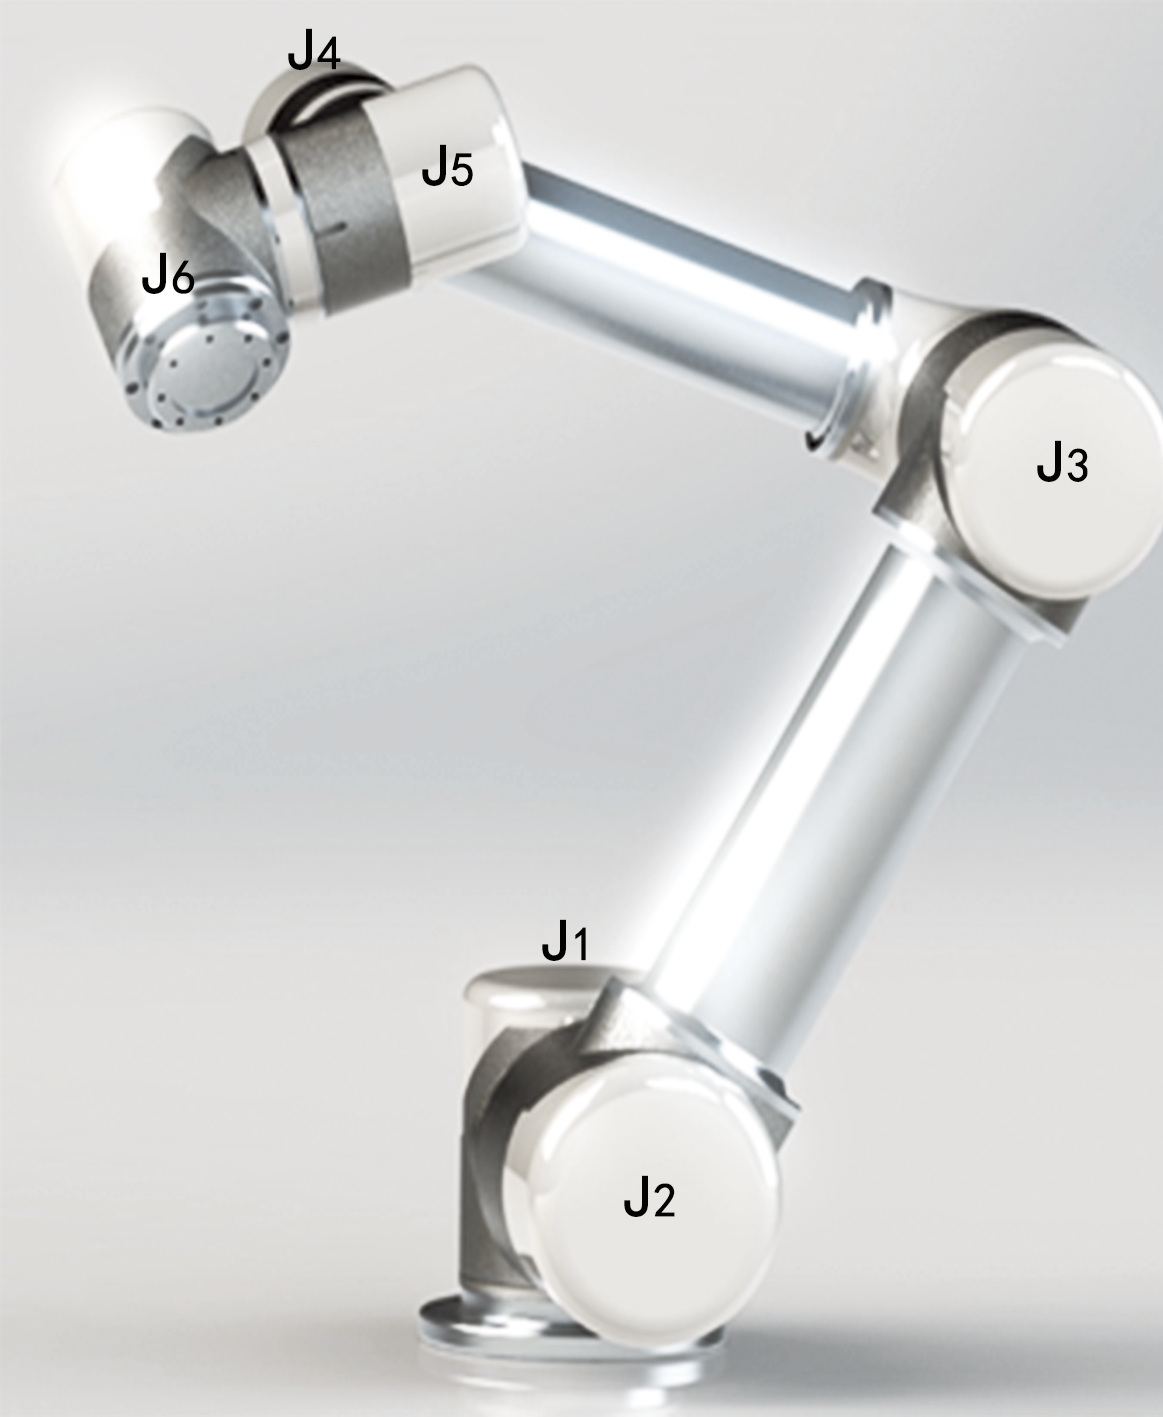
\includegraphics[width=0.35\textwidth ]{ch5-ur-robot.png}\\	 % e.g.,[scale=0.75], [width=0.75\textwidth ]
	\caption{一种UR构型的协作机器人}
	\label{fig.robot}
\end{figure}

工程应用中由于建模和测量的不准确,加上负载的变化以及外部扰动的影响,实际上难以获得机器人精确完整的运动学模型。因此机器人的控制系统中存在的不确定性因素主要可以分为两类,第一类是参数不确定性,如负载质量、连杆长度、连杆质心等物理量未知或部分已知;第二类是非参数不确定性,如高频未建模动态,包括驱动器动力学、结构共振模式,以及低频难以建模动态,如动态/静态摩擦力、关节柔性等。

\subsection{伺服电机控制问题}

\section{仿真实例}

\section{本章总结}
本章主要介绍了

%%==================================================
%% conclusion.tex for BIT Master Thesis
%% modified by yang yating
%% version: 0.1
%% last update: Dec 25th, 2016
%%==================================================

\begin{conclusion}

系统存在不确定性,一直是控制理论研究和工程应用的难点,特别是在离散时间控制中。本文针对一般同时具有参数和非参数不确定性的离散时间被控对象,在已有半参数理论的基础上,研究并完善半参数建模与分析、估计与控制方法,充分利用了系统的先验信息和输入输出历史数据,提高了离散时间控制的实时性和准确性。本文的主要工作总结如下:
\begin{enumerate}
\item 对反馈控制、非线性控制和自适应控制的发展历程、主要趋势和技术特点进行了系统的归纳和总结,指出了最小二乘等线性估计方法的不足,研究了人工神经网络在非线性建模与控制中的应用与难点,介绍了超限学习机,一种在前馈神经网络的实时性应用中具有很大潜力的方法。
\item从回顾反馈机制能力极限等前沿问题出发,针对系统具有参数不确定性和非参数不确定性的特点进行了分析,将系统分为参数描述的线性部分和非参数描述的非线性部分,概括出了一种半参数建模方法,并对实际系统常用的先验信息进行了数学描述。
\item 研究了一种充分利用先验信息的、基于集合的自适应估计方法,即信息浓缩估计,用于解决半参数系统的参数不确定性部分的估计;设计了二维情形下的具体实现算法和步骤,并在数值仿真实验中测试和验证实际效果;归纳总结了信息浓缩估计算法的优缺点,提出了一些计算复杂度问题的优化方向。
\item 介绍了半参数自适应估计与控制问题的一般描述,围绕解决神经网络中经典迭代学习算法的实时性等问题,阐述了超限学习机及其变体的算法特点与非线性建模思路;将超限学习机引入到半参数系统的非参数部分估计中,设计了基于超限学习机的半参数自适应控制算法,并通过仿真实验进行了验证。
\item 在机器人与伺服电机等运动体的轨迹跟踪控制中存在大量的不确定性,将基于信息浓缩估计和超限学习机的半参数建模、估计与控制方法应用到机器人场景中伺服电机的控制问题中,对运动控制问题进行了定制化设计;在仿真实验中进行算法验证,结果表明半参数自适应控制大大提高了轨迹跟踪精度。
\end{enumerate}

基于超限学习机的半参数自适应控制算法的特点主要体现在,充分利用原有系统的先验信息和输入输出历史数据,结合信息浓缩估计和超限学习机等高效且新颖的算法,其建模与控制思路在解决具有较大不确定性的被控对象时具有一般性与通用性。但是,由于控制中利用的估计算法本身的不足,还有一些问题需要进一步研究与完善:
\begin{enumerate}
\item 信息浓缩估计算法的完善。本文目前设计了二维情形下的信息浓缩估计算法,并在自适应运动控制中进行了验证。二维情形可以在一定程度上,解决大量运动控制场景如伺服电机的跟踪控制问题,但是对于涉及到高阶模型,含有多个参数的情况如机器人末端的力反馈控制等问题,可能需要进一步设计高维情形中的信息浓缩估计算法,但核心思路不变。
\item 多变量系统的自适应控制实现。本文主要涉及到控制输入和测量输出都是单一变量的情形,多输入多输出情形的建模与分析思路与本文大致相同,只是涉及到更多变量的信息浓缩估计与神经网路计算,可能需要考虑到本文第三章论述的有关计算复杂度相关的优化策略。
\end{enumerate}
%end of conclusion
\end{conclusion}

%% 参考文献,五号字,使用 BibTeX,包含参考文献文件.bib

%\bibliography{reference/chap1,reference/chap2} %多个章节的参考文献
\bibliography{reference/all}


%%%%%%%%%%%%%%%%%%%%%%%%%%%%%%
%% 后置部分
%%%%%%%%%%%%%%%%%%%%%%%%%%%%%%

%% 附录(章节编号重新计算,使用字母进行编号)
\appendix
\renewcommand\theequation{\Alph{chapter}--\arabic{equation}}  % 附录中编号形式是"A-1"的样子
\renewcommand\thefigure{\Alph{chapter}--\arabic{figure}}
\renewcommand\thetable{\Alph{chapter}--\arabic{table}}

%\include{chapters/app1} 
%\include{chapters/app2}

%(其后部分无编号)
\backmatter

% 发表文章目录
%%==================================================
%% pub.tex for BIT Master Thesis
%% modified by yang yating
%% version: 0.1
%% last update: Dec 25th, 2016
%%==================================================

\begin{publications}{99}
\section*{学术论文}
\begin{enumerate}%
\item *, *, *. 例说自适应控制:从倒立摆谈起. 系统与控制纵横, 3(1), 2016. (期刊)
\item *, *, *. Semi-parametric Adaptive Control of Discrete-time Systems Using Extreme Learning Machine[C].The 9th International Conference on Modelling, Identification, Control, 2017.(EI检索会议,ICMIC2017最佳论文入围奖)
\item *, *, *. Sampled Adaptive Control for Multi-joint Robotic Manipulator with Force Uncertainties[C]. Intelligent Robotics, Applications, 2016.(EI检索会议)
\item *, *, *. Stochastic Adaptive Control of Semi-flexible Robotic Manipulator[C]. 2016 International conference on Advanced Robotics, Intelligent Systems, 2016.(EI检索会议)
\item *, *, *. Driving servo slave station based on EtherCAT with Linux IGH master station[C]. Proceedings of International Symposium on Computational Intelligence and Industrial Applications, 2016.(EI检索会议)
\end{enumerate}

\section*{发明专利}
\begin{enumerate}%
\item *, *, *, *. 一种半柔性机械臂系统的控制方法[P], 201710149827.(已受理)
\item *, *, *, *. 基于Kinect骨骼追踪和无标定视觉伺服的人机协作系统[P], 201611106214.(已受理)
\item *, *, *, *. 一种基于iBeacon的室内定位系统及方法[P], 201610587299.(已受理)
\end{enumerate}

\section*{项目经历}
\begin{enumerate}
\item 国家自然科学基金-面上项目(61473038):大范围不确定随机线性系统自适应滤波估计及其若干应用,2015/01到2018/12,参与.
\item 国家自然科学基金-重大研究计划(91648117):基于数据驱动适应学习的人-机-环境多模态感知与自然交互,2017/01到2019/12,参与.
\item 北京市自然科学基金-面上项目(4172055):基于极限学习机的数据驱动受限约束自适应学习与控制,2017/01到2019/12,参与.
\end{enumerate}
\end{publications}

%\item\textsc{Hao Zhou, Hongbin Ma, Nannan Li, Chenguang Yang}. {Semi-parametric Adaptive Control of Discrete-time Systems Using Extreme Learning Machine}[C].The 9th International Conference on Modelling, Identification, Control, 2017.(EI检索会议)
%\item\textsc{Hao Zhou, Hongbin Ma*, Haiyang Zhan, Yimeng Lei}. {Sampled Adaptive Control for Multi-joint Robotic Manipulator with Force Uncertainties}[C]. Intelligent Robotics, Applications, 2016.(EI检索会议)
%\item\textsc{Hao Zhou, Hongbin Ma*, Dong Wang, Sunjie Chen}. {Stochastic Adaptive Control of Semi-flexible Robotic Manipulator}[C], 2016. 2016 International conference on Advanced Robotics, Intelligent Systems, 2016.(EI检索会议)
%\item Nannan Li, Qing Fei, Hongbin Ma, Sunjie Chen, Hao Zhou. Driving servo slave station based on EtherCAT with Linux IGH master station[C]. Proceedings of International Symposium on Computational Intelligence and Industrial Applications, 2016.(EI检索会议)
%\item 马宏宾, 张星红, 周浩. 例说自适应控制:从道理摆谈起. 系统与控制纵横, 3(1), 2016. (期刊)
% \item\textsc{ 马宏宾, 王冬, 周浩, 陈孙杰}. {一种基于iBeacon的室内定位系统及方法}[P]. 2016.(发明专利,已受理)
%\item\textsc{马宏宾, 王浩, 周浩, 陈孙杰}. {基于Kinect骨骼追踪和无标定视觉伺服的人机协作系统}[P]. 2016.(发明专利,已受理)
%\item\textsc{周浩, 马宏宾, 陈孙杰, 李楠楠}. {一种半柔性机械臂系统的控制方法}[P]. 2017.(发明专利,已受理)

% 致谢
%%==================================================
%% thanks.tex for BIT Master Thesis
%% modified by yang yating
%% version: 0.1
%% last update: Dec 25th, 2016
%%==================================================

\begin{thanks}

本论文的工作是在导师***教授的指导下独立完成的。两年半的时光匆匆划过,虽有苦有泪,但它始终是我这一生中一段重要的旅程。研究生阶段让我在更好的完善自己的同时,也丰富了我的知识,开阔了眼界。而如今,我能够顺利的完成我的毕业论文,也是因为一直有那些人陪伴在我的左右,在我错误时指导我,在我失意时陪伴我,在我受挫时鼓励我的那些人。感谢你们一路上的指引和教导,让我有了今天的成就!

首先,我要感谢敬爱的导师***教授。

在此,我也要特别感谢我的父母及其他亲人,你们的支持和帮助,一直是我前进的动力,能够顺利完成硕士学位,也离不开你们在经济上的支持,感恩你们无私的爱!

最后,感谢本论文中所引用的参考文献的作者,你们的文章给了我无限的启迪和智慧,感谢本论文的评审老师和答辩委员会老师,同时也感谢自动化学院的所有任课老师们,感谢各位老师的不惜吝教。

\end{thanks}

% 作者简介(博士论文需要)
%\include{chapters/resume}

\end{document}
